% DO NOT COMPILE THIS FILE DIRECTLY!
% This is included by the other .tex files.

\begin{frame}[t,plain]
\titlepage
\end{frame}

\begin{frame}
\frametitle{Who we are - MISP and CIRCL}
\begin{itemize}
\item CIRCL is mandated by the Ministry of Economy and acting as the Luxembourg National CERT for private sector.
\item {\bf CIRCL leads the development} of the Open Source MISP threat intelligence platform which is used by many military or intelligence communities, private companies, financial sector, National CERTs and LEAs globally.
\item {\bf CIRCL runs multiple large MISP communities performing active daily threat-intelligence sharing}.
\item Funding is shared between Luxembourg, several European Union programs and partnerships (EU/US) agreements.
\end{itemize}
\end{frame}
\begin{frame}
	\frametitle{Plan}
	\begin{itemize}
		\item An introduction to the MISP project and how it supports ISACs.
        \item Building an information sharing community, lessons learnt and best practices\footnote{We published the complete guidelines in \url{https://www.x-isac.org/assets/images/guidelines_to_set-up_an_ISAC.pdf}}.
	\end{itemize}
\end{frame}

\begin{frame}
        \frametitle{MISP Project Overview}
        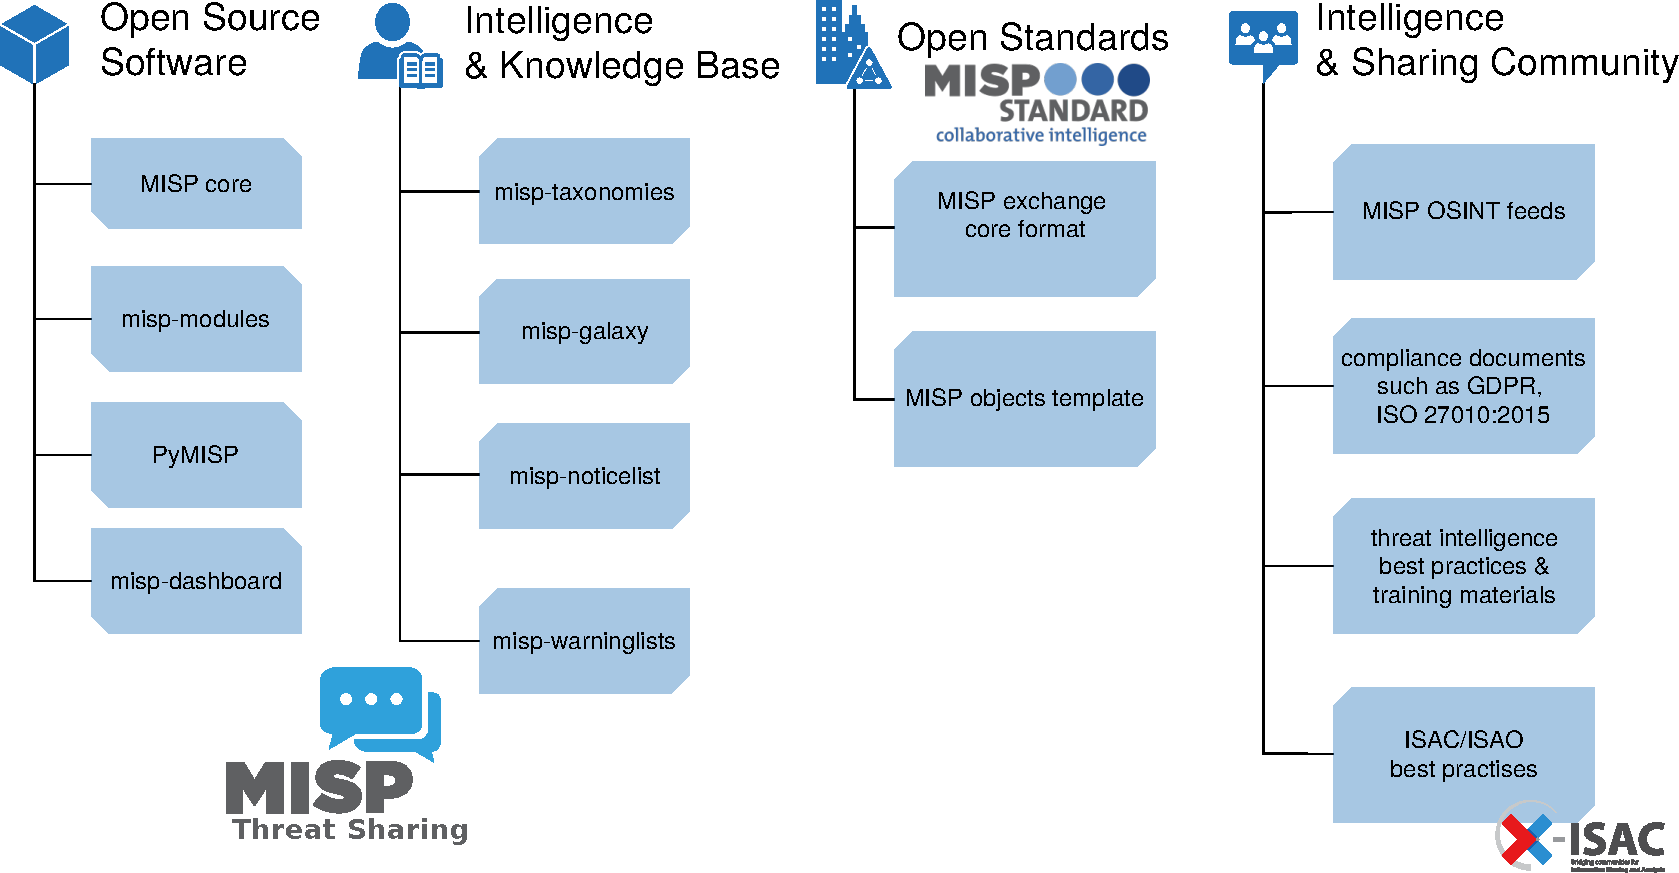
\includegraphics[scale=0.35]{misp-overview-simplified.pdf}
\end{frame}

\begin{frame}
    \frametitle{MISP features}
    \begin{itemize}
            \item MISP project is an open source project developed the past 10-year with a large and active community.
            \item A complete set of features in MISP to work as a {\bf threat intelligence platform} with a strong set of {\bf information sharing capabilities}. 
            \item A {\bf flexible information sharing} model to support centralised, distributed or mixed model ISACs.
            \item Integration and extensability functionalities allow MISP to support different use-cases (from cybersecurity to complex intelligence community requirements).
    \end{itemize}
\end{frame}

\begin{frame}
    \frametitle{MISP feature - correlation}
    \begin{itemize}
        \item MISP includes a {\bf powerful engine for correlation} which allows analysts to discover correlating values between attributes. 
        \item Getting a direct benefit from shared information by other ISAC members.
    \end{itemize}
    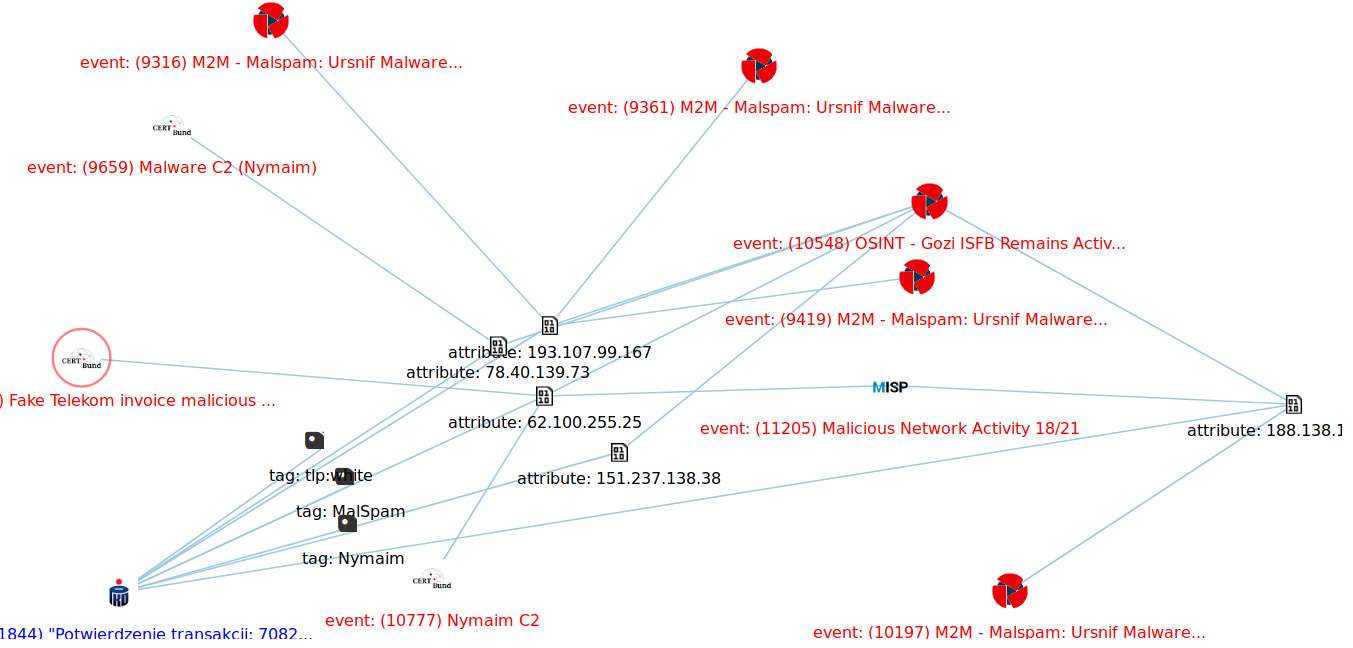
\includegraphics[scale=0.20]{campaign.png}
\end{frame}

\begin{frame}
    \frametitle{MISP feature - event graph}
    \begin{itemize}
        \item {\bf Analysts can create stories} based on graph relationships between objects, attributes.
         \item ISACs users can directly understand the information shared.
    \end{itemize}
    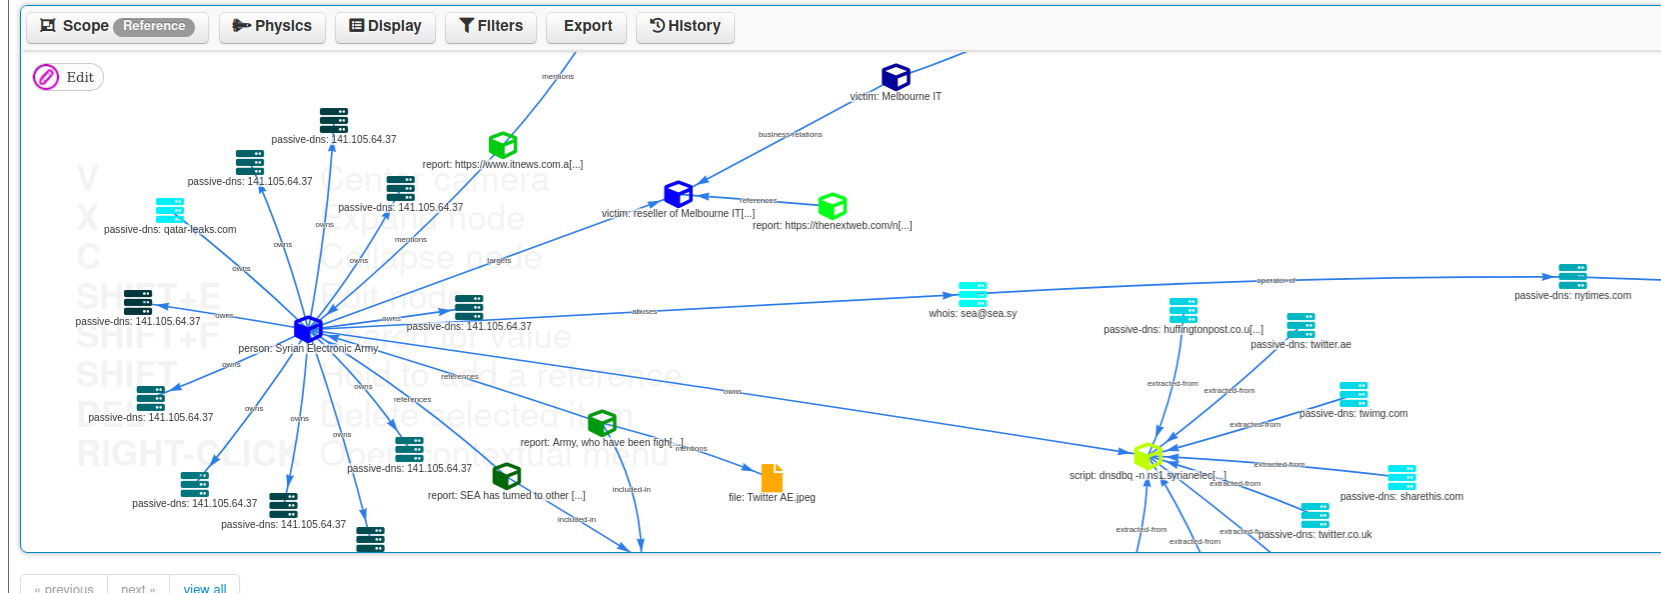
\includegraphics[scale=0.20]{event-graph.png}
\end{frame}

\begin{frame}
    \frametitle{MISP feature - workflow}
    \begin{itemize}
        \item MISP can control publication steps via {\bf customised workflow} when publishing events, creating new users... 
        \item ISACs can enforce specific policies and rules via workflows.  
    \end{itemize}
    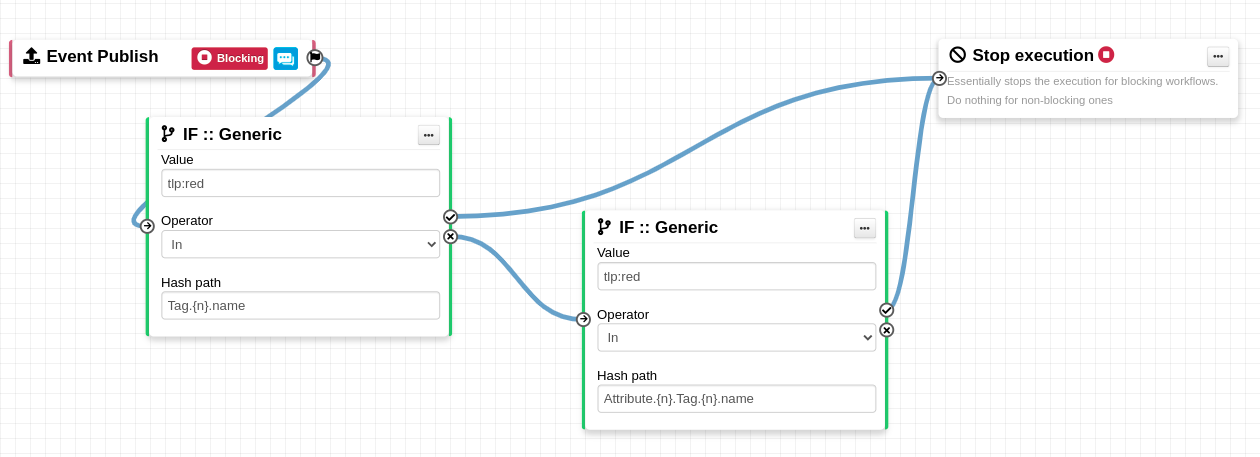
\includegraphics[scale=0.20]{workflow.png}
\end{frame}

\begin{frame}
    \frametitle{MISP feature - flexible data models} 
    \begin{itemize}
        \item MISP can be easily customised to support other data models (via {\bf object templates, taxonomies and galaxies}).
        \item ISACs don't need to change their models, policies or structure.
        \item A library of {\bf 290+ objects, 200+ taxonomies and many galaxies} (such as MITRE ATT\&CK) are available. 
    \end{itemize}
    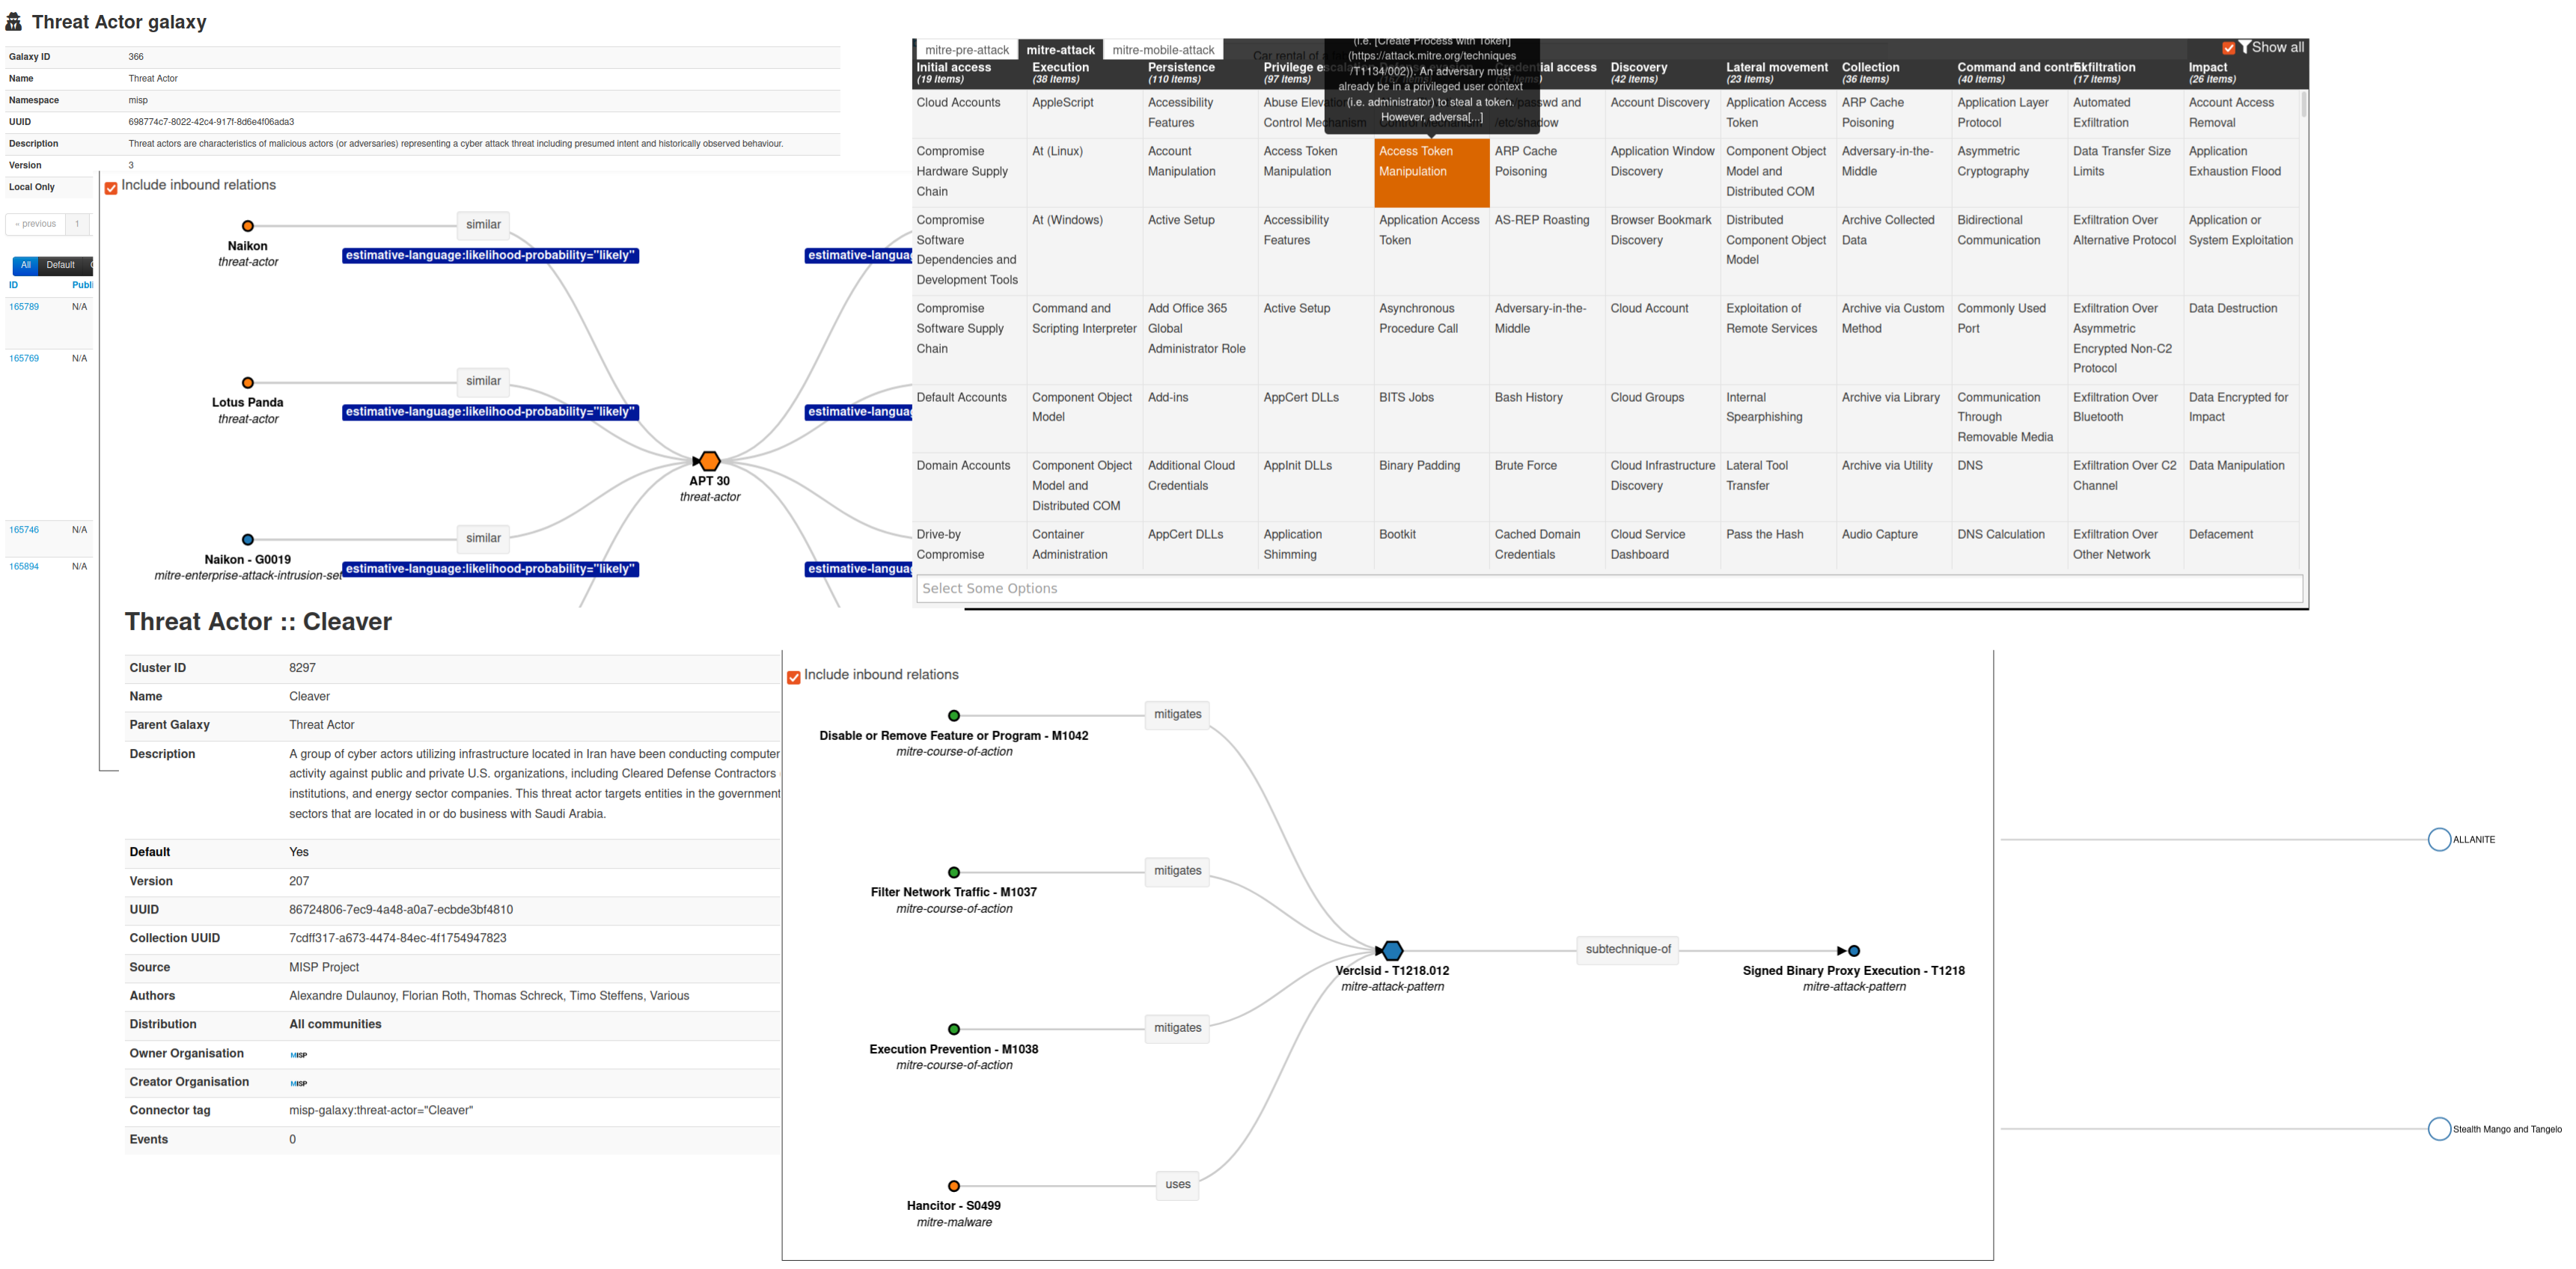
\includegraphics[scale=0.12]{galaxy.png}
\end{frame}


\begin{frame}
\frametitle{Communities operated by CIRCL}
\begin{itemize}
        \item As a CSIRT, CIRCL operates a wide range of communities
        \item We use it as an {\bf internal tool} to cover various day-to-day activities
        \item Whilst being the main driving force behind the development, we're also one of the largest consumers
	\item Different communities have different needs and restrictions
\end{itemize}
\end{frame}

\begin{frame}
\frametitle{Communities operated by CIRCL}
\begin{itemize}
        \item Private sector community
	\begin{itemize}
		\item Our largest sharing community
		\item Over {\bf +1500 organisations}
		\item {\bf +4000 users}
		\item Functions as a central hub for a lot of different sharing communities
		\item Private organisations, researchers, various SoCs, some CSIRTs, etc
	\end{itemize}
	\item CSIRT community
	\begin{itemize}
		\item Tighter community
		\item National CSIRTs, connections to international organisations, etc
	\end{itemize}
\end{itemize}
\end{frame}

\begin{frame}
\frametitle{Communities co-operated and supported by CIRCL}
\begin{itemize}
	\item Financial sector community
	\begin{itemize}
		\item Banks, payment processors, etc.
		\item Sharing of {\bf mule accounts} and {\bf non-cyber threat information}
	\end{itemize}
    \item X-ISAC\footnote{\url{https://www.x-isac.org/}}
	\begin{itemize}
		\item {\bf Bridging the gap} between the various sectorial and geographical ISACs
		\item New, but ambitious initiative
		\item Goal is to {\bf bootstrap the cross-sectorial sharing} along with building the infrastructure to enable sharing when needed
	\end{itemize}
\end{itemize}
\end{frame}

\begin{frame}
\frametitle{Communities supported by CIRCL}
\begin{itemize}
        \item ISAC / specialised community MISPs
        \begin{itemize}
            \item Topical or community specific instances hosted or co-managed by CIRCL
            \item Examples, GSMA, FIRST.org, CSIRT network, PISAX.org, etc
            \item Often come with their {\bf own taxonomies and domain specific object definitions}
        \end{itemize}
	\item FIRST.org's MISP community
	\item Telecom and Mobile operators' such as GSMA T-ISAC community
	\item Various ad-hoc communities for exercises for example
	\begin{itemize}
		\item The ENISA exercise for example
         \item Locked Shields exercise
	\end{itemize}
\end{itemize}
\end{frame}

\begin{frame}
\frametitle{Sharing Scenarios in MISP}
\begin{itemize}
	\item Sharing can happen for {\bf many different reasons}. Let's see what we believe are the typical CSIRT scenarios
        \item We can generally split these activities into 4 main groups when we're talking about traditional CSIRT tasks:
	\begin{itemize}
		\item Core services
		\item Proactive services
		\item Advanced services
		\item Sharing communities managed by CSIRTs for various tasks
	\end{itemize}
\end{itemize}
\end{frame}

\begin{frame}
\frametitle{CSIRT core services}
\begin{itemize}
	\item Incident response
	\begin{itemize}
		\item {\bf Internal storage} of incident response data
		\item Sharing of indicators {\bf derived from incident response}
		\item {\bf Correlating data} derived and using the built in analysis tools
		\item {\bf Enrichment} services
		\item {\bf Collaboration} with affected parties via MISP during IR
		\item {\bf Co-ordination} and collaboration
		\item {\bf Takedown} requests
	\end{itemize}
	\item Alerting of information leaks (integration with {\bf AIL}\footnote{\url{https://www.ail-project.org/}})
\end{itemize}
\end{frame}

\begin{frame}
\frametitle{CSIRT proactive services}
\begin{itemize}
	\item {\bf Contextualising} both internal and external data
	\item {\bf Collection} and {\bf dissimination} of data from various sources (including OSINT)
	\item Storing, correlating and sharing own manual research ({\bf reversing, behavioural analysis})
	\item Aggregating automated collection ({\bf sandboxing, honeypots, spamtraps, sensors})
	\begin{itemize}
		\item MISP allows for the creation of {\bf internal MISP "clouds"}
		\item Store {\bf large specialised datasets} (for example honeypot data)
		\item MISP has {\bf interactions with} a large set of such {\bf tools} (Cuckoo, Mail2MISP, etc)
	\end{itemize}
	\item {\bf Situational awareness} tools to monitor trends and adversary TTPs within my sector/geographical region (MISP-dashboard, built in statistics)
\end{itemize}
\end{frame}

%\begin{frame}
%\frametitle{CSIRT proactive services - MISP dashboard}
%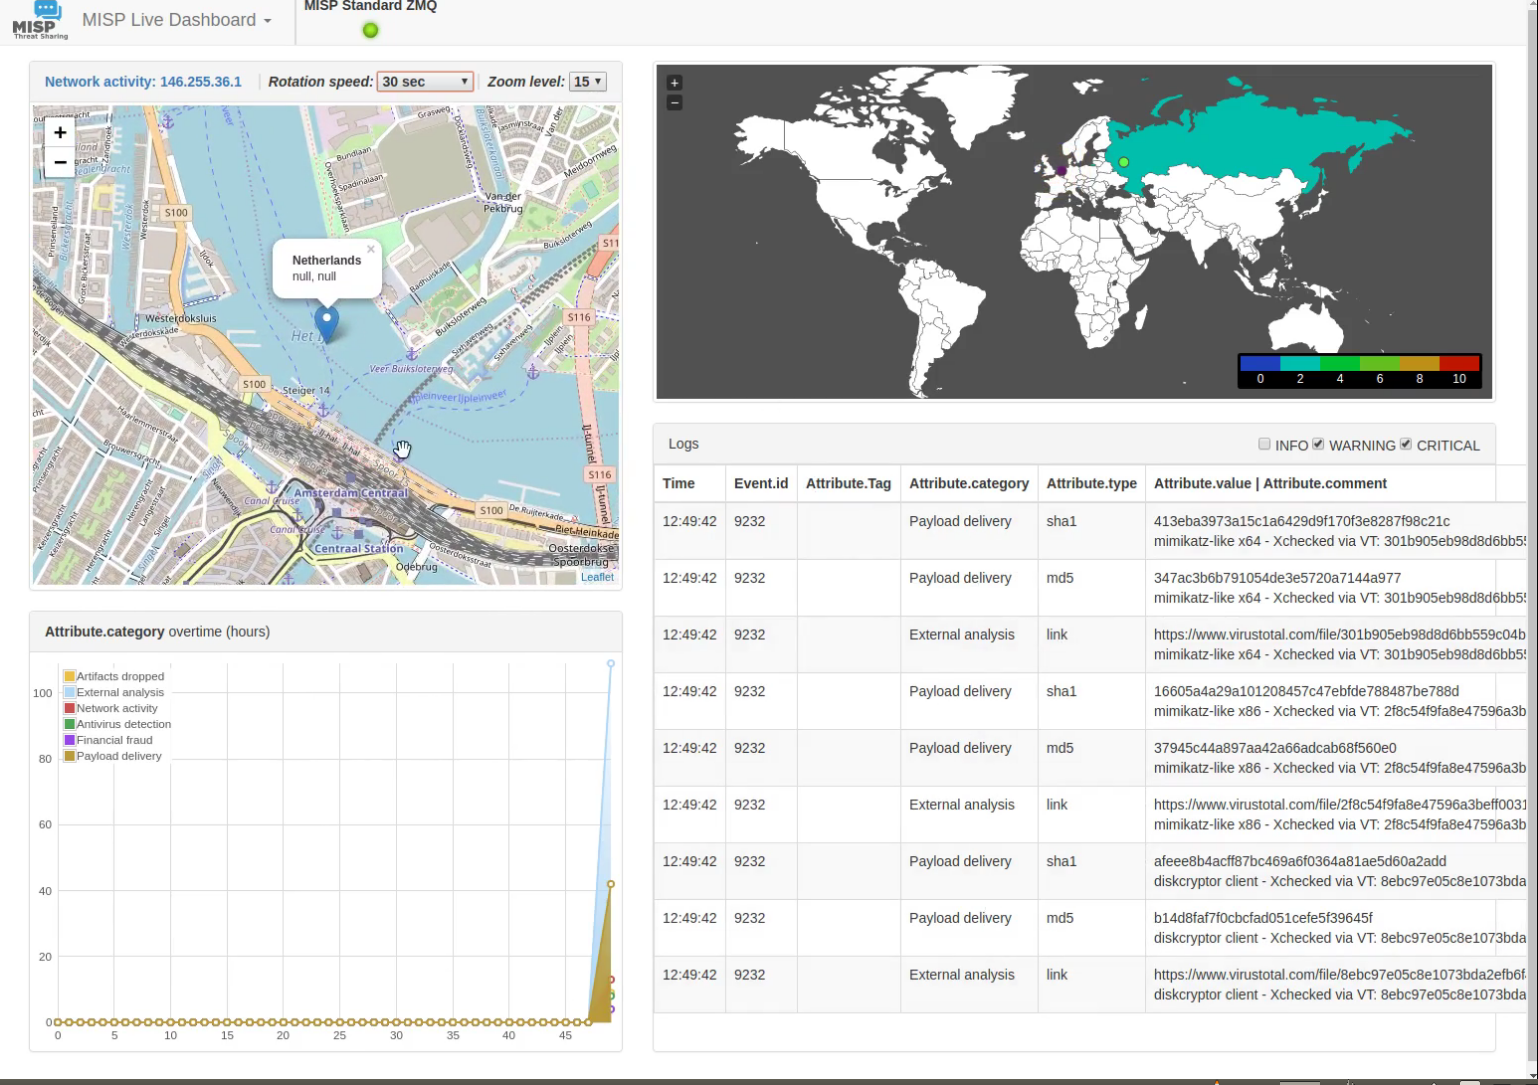
\includegraphics[scale=0.18]{screenshots/dashboard-live.png}
%\end{frame}

%\begin{frame}
%\frametitle{CSIRT proactive services - MISP dashboard}
%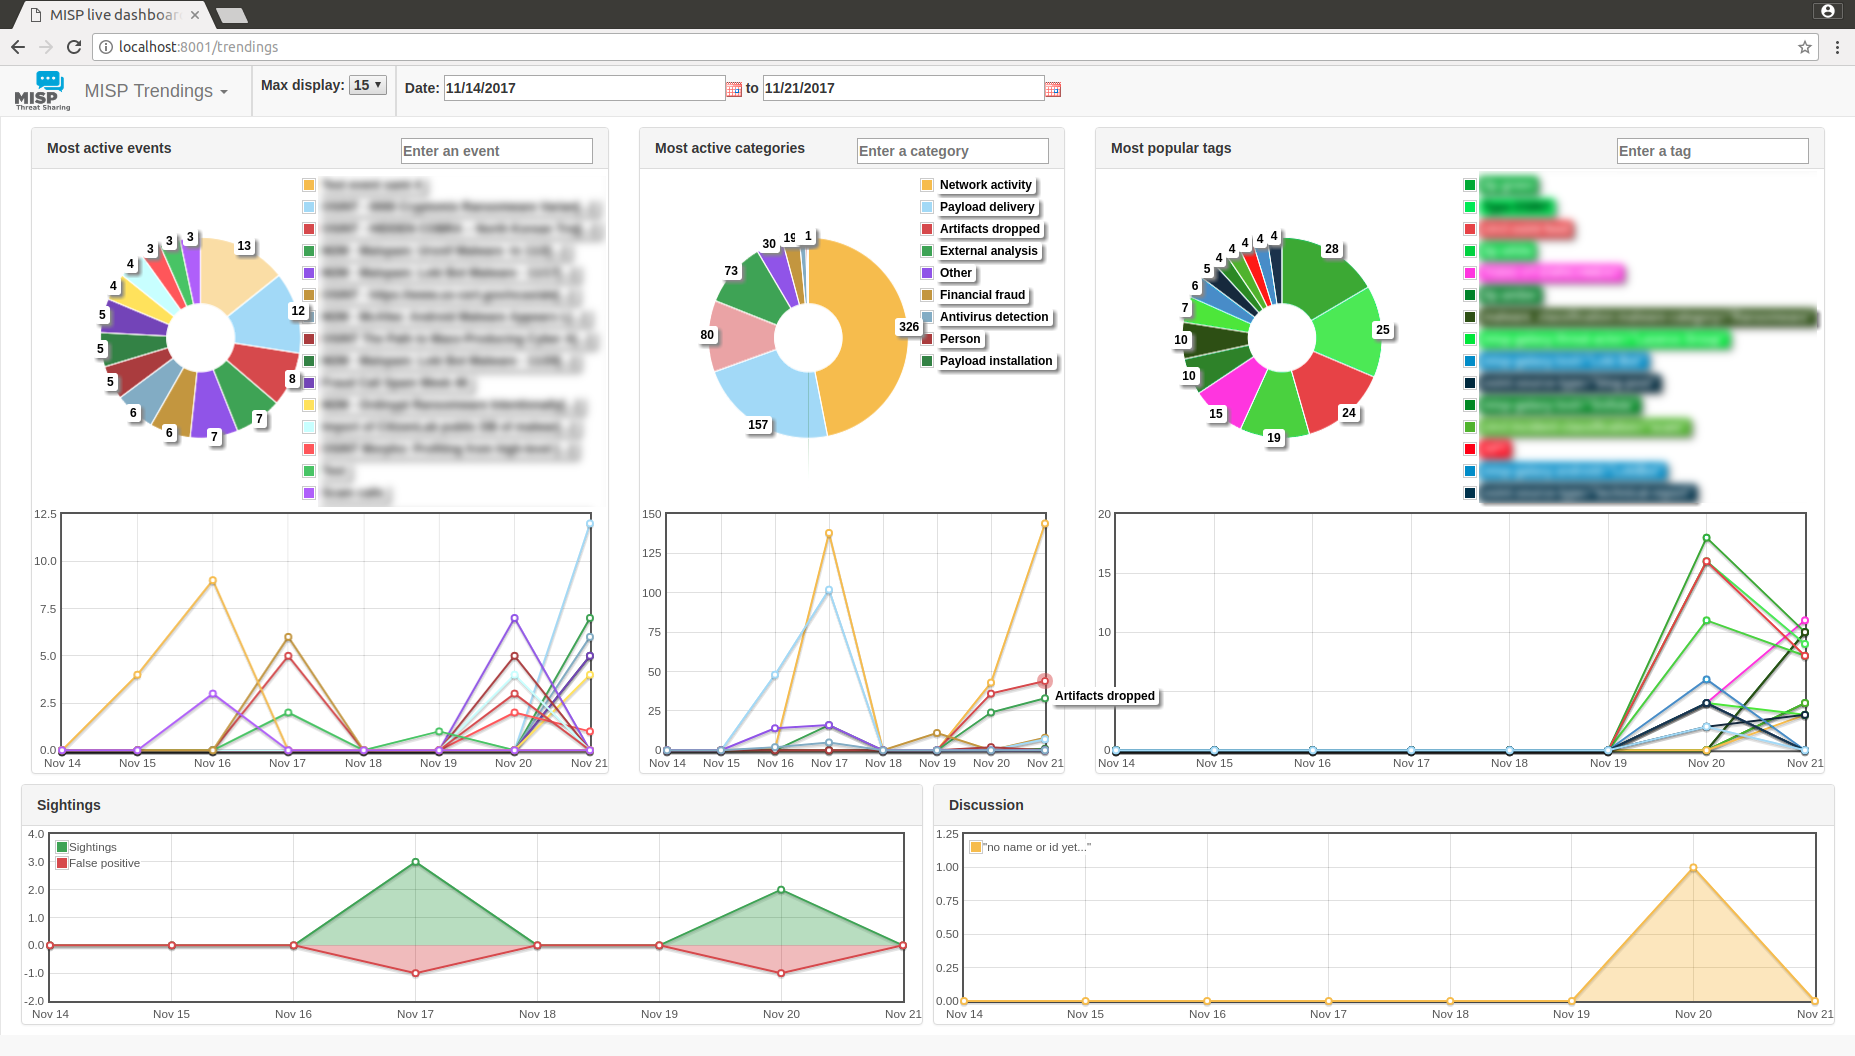
\includegraphics[scale=0.18]{screenshots/dashboard-trendings.png}
%\end{frame}

\begin{frame}
\frametitle{CSIRT advanced services}
\begin{itemize}
	\item Supporting {\bf forensic analysts}
	\item Collaboration with {\bf law enforcement}
	\item {\bf Vulnerability} information sharing
	\begin{itemize}
		\item {\bf Notifications} to the constituency about relevant vulnerabilities
		\item {\bf Co-ordinating} with vendors for notifications (*)
		\item Internal / closed community sharing of pentest results
	\end{itemize}
\end{itemize}
\end{frame}


\begin{frame}
\frametitle{ISACs and CSIRT role in information sharing}
\begin{itemize}
	\item {\bf Reporting} non-identifying information about incidents (such as outlined in NISD)
	\item {\bf Seeking} and engaging in {\bf collaboration} with CSIRT or other parties during an incident
	\item Pre-sharing information to {\bf request for help} / additional information from the community
	\item {\bf Pseudo-anonymised sharing} through 3rd parties to {\bf avoid attribution} of a potential target
	\item Building processes for {\bf other types of sharing} to get the community engaged and acquainted with the methodologies of sharing (mule account information, disinformation campaigns, border control, etc)
\end{itemize}
\end{frame}

\begin{frame}
\frametitle{Compliance, legal framework and ISACs}
\begin{itemize}
	\item MISP project collaborated with legal advisory services
	\begin{itemize}
		\item Information sharing and cooperation {\bf enabled by GDPR};
		\item How MISP enables stakeholders identified by the {\bf NISD} to perform key activities;
        \item {\bf ISO/IEC 27010:2015} - Information security management for inter-sector and inter-organizational communications;
        \item Guidelines to setting up an information sharing community such as an ISAC or ISAO;
	\end{itemize}
	\item For more information: https://www.misp-project.org/compliance/
\end{itemize}
\end{frame}

\begin{frame}
\frametitle{Getting started with building your own sharing community}
\begin{itemize}
	\item Starting a sharing community is {\bf both easy and difficult} at the same time
    \item Many moving parts and most importantly, you'll be dealing with a {\bf diverse group of people}
	\item Understanding and working with your constituents to help them face their challenges is key
\end{itemize}
\end{frame}

\begin{frame}
\frametitle{Running a sharing community using MISP - How to get going?}
\begin{itemize}
	\item Different models for constituents
	\begin{itemize}
        \item {\bf Connecting to} a MISP instance hosted by a ISAC 
        \item {\bf Hosting} their own instance and connecting to ISAC's MISP
        \item {\bf Becoming member} of a sectorial MISP community that is connected to ISAC's community
	\end{itemize}
	\item Planning ahead for future growth
	\begin{itemize}
		\item Estimating requirements
		\item Deciding early on common vocabularies
		\item Offering services through MISP
	\end{itemize}
\end{itemize}
\end{frame}

\begin{frame}
\frametitle{Rely on our instincts to immitate over expecting adherence to rules}
\begin{itemize}
    \item {\bf Lead by example} - the power of immitation
    \item Encourage {\bf improving by doing} instead of blocking sharing with unrealistic quality controls
	\begin{itemize}
		\item What should the information look like?
		\item How should it be contextualise
		\item What do you consider as useful information?
		\item What tools did you use to get your conclusions?
        \item How the information could be used by the ISAC members?
	\end{itemize}
\item Side effect is that you will end up {\bf raising the capabilities of your constituents}
\end{itemize}
\end{frame}

\begin{frame}
\frametitle{What counts as valuable data?}
\begin{itemize}
	\item Sharing comes in many shapes and sizes
	\begin{itemize}
		\item Sharing results / reports is the classical example
		\item Sharing enhancements to existing data
		\item Validating data / flagging false positives
		\item Asking for support from the community
	\end{itemize}
\item {\bf Embrace all of them}. Even the ones that don't make sense right now, you never know when they come handy...
\end{itemize}
\end{frame}

\begin{frame}
\frametitle{How to deal with organisations that only "leech"?}
\begin{itemize}
    \item From our own communities, only about {\bf 30\%} of the organisations {\bf actively share data}
	\item We have come across some communities with sharing requirements
	\item In our experience, this sets you up for failure because:
	\begin{itemize}
		\item Organisations losing access are the ones who would possibily benefit the most from it
		\item Organisations that want to stay above the thresholds will start sharing junk / fake data
		\item You lose organisations that might turn into valuable contributors in the future
	\end{itemize}
\end{itemize}
\end{frame}

\begin{frame}
\frametitle{So how does one convert the passive organisations into actively sharing ones?}
\begin{itemize}
    \item Rely on {\bf organic growth} and it takes time (+2 years is common)
    \item {\bf Help} them increase their capabilities
	\item As mentioned before, lead by example
	\item Rely on the inherent value to one's self when sharing information (validation, enrichments, correlations)
    \item {\bf Give credit} where credit is due, never steal the contributions of your community (that is incredibly demotivating)
\end{itemize}
\end{frame}

\begin{frame}
\frametitle{Dispelling the myths around blockers when it comes to information sharing}
        \begin{itemize}
                \item Sharing difficulties are not really technical issues but often it's a matter of {\bf social interactions} (e.g. {\bf trust}).
		\begin{itemize}
			\item You can play a role here: organise regular workshops, conferences, have face to face meetings
		\end{itemize}
                \item Legal restrictions
                        \begin{itemize}
                                \item "Our legal framework doesn't allow us to share information."
                                \item "Risk of information leak is too high and it's too risky for our organization or partners."
                        \end{itemize}
                \item Practical restrictions
                        \begin{itemize}
                                \item "We don't have information to share."
                                \item "We don't have time to process or contribute indicators."
                                \item "Our model of classification doesn't fit your model."
                                \item "Tools for sharing information are tied to a specific format, we use a different one."
                        \end{itemize}
        \end{itemize}
\end{frame}

\begin{frame}
\frametitle{Contextualising the information}
\begin{itemize}
    \item Sharing {\bf technical information} is a {\bf great start}
	\item However, to truly create valueable information for your community, always consider the context:
	\begin{itemize}
		\item Your IDS might not care why it should alert on a rule
		\item But your analysts will be interested in the threat landscape and the "big picture"
	\end{itemize}
    \item Classify data to make sure your partners understand why it is {\bf important for you}, so they can see why it could be {\bf useful to them}
    \item Massively important once an organisation has the maturity to filter the most critical {\bf subsets of information for their own defense}
\end{itemize}
\end{frame}

\begin{frame}
\frametitle{Choice of vocabularies}
\begin{itemize}
    \item MISP has a verify {\bf versatile system} (taxonomies) for classifying and marking data
	\item However, this includes different vocabularies with obvious overlaps
    \item MISP allows you to {\bf pick and choose vocabularies} to use and enforce in a community
	\item Good idea to start with this process early
	\item If you don't find what you're looking for:
	\begin{itemize}
		\item Create your own (JSON format, no coding skills required)
		\item If it makes sense, share it with us via a pull request for redistribution
	\end{itemize}
\end{itemize}
\end{frame}

\begin{frame}
\frametitle{Conclusion}
    \begin{itemize}
        \item MISP is a complete and advanced open source stack available to create large international sharing communities (JP/US/EU).
        \item Building and improving ISACs is critical to limit the impact of security threats.
        \item We welcome partnerships in the field of information sharing.
    \end{itemize}
\end{frame}


\begin{frame}
\frametitle{Get in touch if you need some help to get started}
\begin{itemize}
\item Getting started with building a new community can be daunting. Feel free to get in touch with us if you have any questions!
\item Contact: info@circl.lu
\item \url{https://www.circl.lu/}
\item \url{https://github.com/MISP}  \url{https://www.misp-project.org/}  \url{https://twitter.com/MISPProject}
\end{itemize}
\end{frame}

\begin{frame}
\frametitle{Backup slides}
{\center Backup slides}
\end{frame}

\begin{frame}
\frametitle{Shared libraries of meta-information (Galaxies)}
\begin{itemize}
    \item The MISPProject in co-operation with partners provides a {\bf curated list of galaxy information}
	\item Can include information packages of different types, for example:
	\begin{itemize}
        \item Threat actor information (event different models or approaches)
		\item Specialised information such as Ransomware, Exploit kits, etc
		\item Methodology information such as preventative actions
		\item Classification systems for methodologies used by adversaries - ATT\&CK
	\end{itemize}
	\item Consider improving the default libraries or contributing your own (simple JSON format)
    \item If there is something you cannot share, run your own galaxies and {\bf share it out of bound} with partners
	\item Pull requests are always welcome
\end{itemize}
\end{frame}

\begin{frame}
\frametitle{False-positive handling}
\begin{itemize}
	\item You might often fall into the trap of discarding seemingly "junk" data
	\item Besides volume limitations (which are absolutely valid, fear of false-positives is the most common reason why people discard data) - Our recommendation:
	\begin{itemize}
		\item Be lenient when considering what to keep
		\item Be strict when you are feeding tools
	\end{itemize}
\item MISP allows you to {\bf filter out the relevant data on demand} when feeding protective tools
\item What may seem like {\bf junk to you may} be absolutely {\bf critical to other users}
\end{itemize}
\end{frame}

\begin{frame}
\frametitle{False-positive handling}
\begin{itemize}
    \item {\bf Analysts} will often be interested in the {\bf modus operandi} of threat actors over {\bf long periods of time}
	\item Even cleaned up infected hosts might become interesting again (embedded in code, recurring reuse)
	\item Use the tools provided to eliminate obvious false positives instead and limit your data-set to the most relevant sets
\end{itemize}
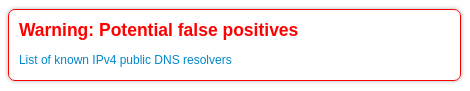
\includegraphics[scale=0.8]{screenshots/false-positive.png}
\end{frame}


